\newpage
\section{Задание 11}

Построить двумерное пуассоновское поле, отвечающее сложному пуассоновскому 
процессу:
\begin{enumerate}
	\item Первая интерпретация: система массового обслуживания. При этом первая 
    координата поля~---~время поступления заявки в СМО (равномерное 
    распределение), вторая~---~время её обслуживания (распределение $\chi^2$ с 
    $10$-ю степенями свободы).

	\item Вторая интерпретация: система массового обслуживания с циклической 
    интенсивностью $\lambda(t) = \lambda_0(1+\cos(t))$ и единичными скачками. 
    Свести данную задачу моделирования неоднородного пуассоновского процесса 
    при помощи метода Льюиса и Шедлера к моделированию двумерного 
    пуассоновского поля, где первая координата имеет равномерное распределение, 
    а вторая~---~распределение Бернулли.
	
	\item Третья интерпретация: работа страховой компании. Первая 
    координата~---~момент наступления страхового случая (равномерное 
    распределение), вторая координата~---~величина ущерба (распределение 
    Парето). Поступление капитала по времени линейно со скоростью $c > 0$, 
    начальный капитал $W > 0$.
	
	\item Для каждой системы рассмотреть всевозможные случаи поведения системы 
    в зависимости от значения параметров.
\end{enumerate}

\subsection{СМО}
    Систему массового обслуживания будем моделировать временами поступления 
    заявок $t_i$: $t_i - t_{i-1} \sim \mathrm{Exp}(\lambda)$, где $\lambda$~--- 
    интенсивность потока заявок, и временами обработки завявок $s_i$ 
    распределенных по закону $\chi^2$ с $10$ степенями свободы. Для каждой 
    заявки будет считаться время ее исполнения, т.е. если следуюзщая заявка 
    пришла раньше чем прошло время обработки заявки то будет накапливаться 
    очередь. Поскольку $\Exp s_i = 10$, в зависимости того, больше $\lambda$ чем
    $\frac{1}{10}$ или меньше, очередь будет в среднем накапливаться или 
    сокращаться соответственно.

\subsection{СМО с циклической интенсивностью}
    Имеющийся неоднородный процесс с помощью вышеупомянутого алгоритма сводится 
    к двумерному пуассоновскому полю, а именно, генерируется стационарный 
    пуассоновский процесс $X_t$, из множества точек роста которого случайно 
    (с бернуллиевским распределением) выбирается подмножество $T$. Совокупность 
    полученных величин образует искомое пуассоновское поле.

    Иллюстрации работы моделей СМО представлены на рис. \ref{smo} 

    \begin{figure}[tbp]
        \centering
        \begin{subfigure}[b]{0.48\textwidth}
            \centering
            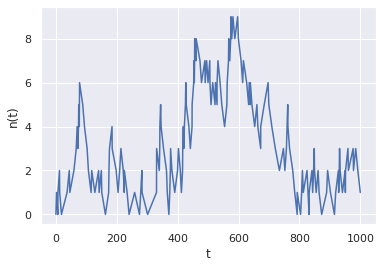
\includegraphics[width=\textwidth]{resources/task11_smo_const.png}
            \caption{с постоянной интенсивностью}
        \end{subfigure}
        \hfill
        \begin{subfigure}[b]{0.48\textwidth}
            \centering
            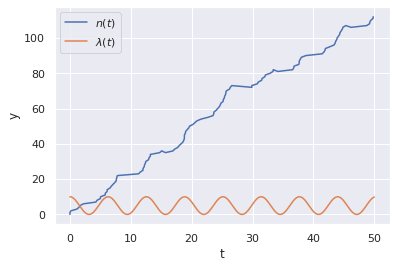
\includegraphics[width=\textwidth]{resources/task11_smo_cyclic.png}
            \caption{с циклической интенсивностью}
        \end{subfigure}
        \caption{СМО}
        \label{smo}
    \end{figure}

\subsection{Работа страховой компании}
    Для построения модели работы страховой компании генерируются времена 
    поступления страховых случаев $t_i$: $t_i - t_{i-1} \sim 
    \mathrm{Exp}(\lambda)$ и ущерб страхового случая $s_i$ распределенный по 
    Парето с параметрами $x_m$ и $k$. По ним можно вычислить величину капитала 
    компании в момент $t$: $W(t) = W_0 + cy - \sum_{i:t_i<t} s_i$ и среднюю 
    скорость прироста капитала $(\Exp W(t))' = c - \dfrac{\lambda k x_m}{k-1}$.
    Из чего можно заключить, что страховая компания будет расти при 
    $c(k-1)-\lambda k x_m > 0$, и обанкротится при $c(k-1)-\lambda k x_m < 0$.

    \begin{figure}[tbp]
        \centering
        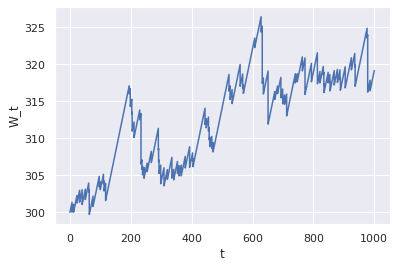
\includegraphics[width=0.5\textwidth]{resources/task11_insur_comp.png}
        \caption{работа страховой компании}
        \label{ins_comp}
    \end{figure}